\documentclass[12pt]{article}
\usepackage{../../../lecture_notes}
\usepackage{../../../math}
\usepackage{../../../uark_colors}

\hypersetup{
  colorlinks = true,
  allcolors = ozark_mountains,
  breaklinks = true,
  bookmarksopen = true
}

\begin{document}
\begin{center}
  {\Huge\bf Final - Fall 2024}
  
  \smallskip
  {\large\it ECON 4753 — University of Arkansas}
\end{center}

\vspace{5mm}

\begin{enumerate}
  \item In this course, we have described a set of methods that are very `flexible' at modeling $y = f(X)$. We have also learned about a simple linear regression model ($y = \alpha + X \beta$). Describe one advantage of each method (a flexible model and a linear model).

  \bigskip
  \item The following regression uses the ``College Scorecard'' which describes all U.S. colleges/universities. The outcome variable is the average annual earnings (\$) of students 10 years after they enroll. The explanatory varaible is the median SAT Math score of the student body. I include both the variable itself and its square (quadratic in SAT math):
  \begin{codeblock}[{}]
OLS estimation, Dep. Var.: mean_earnings_10yr_after
Observations: 935
Standard-errors: Heteroskedasticity-robust 
                          Estimate   Std. Error  t value   Pr(>|t|)    
(Intercept)          108369.503822 19595.243683  5.53040 4.1500e-08 ***
sat_math_median        -337.941666    68.781472 -4.91327 1.0577e-06 ***
I(sat_math_median^2)      0.411678     0.059815  6.88258 1.0783e-11 ***
---
Signif. codes:  0 '***' 0.001 '**' 0.01 '*' 0.05 '.' 0.1 ' ' 1
  \end{codeblock}

  \begin{enumerate}[leftmargin = 2em]
    \item What is the predicted earnings for a school with an average SAT math score of 500 (round to the nearest dollar)? 
    
    \item Say you take a school with an average SAT math score of 500. What is the predicted marginal change in $Y$ for a school with a 1 unit increase in average SAT math score?
  \end{enumerate}
\end{enumerate}
  
\newpage
\begin{enumerate}
  \setcounter{enumi}{2}
  \item Say you have a sample of stores where you observe the average daily revenue and the number of employees on the sales floor. You regress the $\log$ of average daily revenue on the number of employees and estimate a coefficient of $\hat{\beta}_1 = 0.03$ and a standard error of $\text{SE}(\hat{\beta}_1) = 0.005$. 
  \begin{enumerate}
    \item Interpret this coefficient estimate in words.
    
    \item The company does not want to increase the number of staff if these results are not statistically significant. Perform a test of the null that $\beta_1 = 0$. The company is risk adverse and want you to use a level of significance of $\alpha = 0.01$ (the z-score associated with this is $2.58$). 
  \end{enumerate}
  
  \bigskip
  \item For the following questions, we will look at daily bitcoin price data (see Figure 1).
  \begin{enumerate}
    \item Consider conducing inference on this time-series using a 30-day one-sided moving average. How do you think this method would perform on the bitcoin price data? Please explain why.
    
    \item Say, instead, you were to use a flexible piecewise linear function (say 10+ breaks) to forecast future bitcoin prices. Why might you be concerned about extrapolating your regression estimate into the future to predict bitcoin prices.
  \end{enumerate}
\end{enumerate}

\bigskip
\begin{figure}[h!]
  \caption{Daily Closing Prices of Bitcoin}
  \label{fig:bitcoin}
  
  \vspace*{-2\bigskipamount}
  \begin{center}
    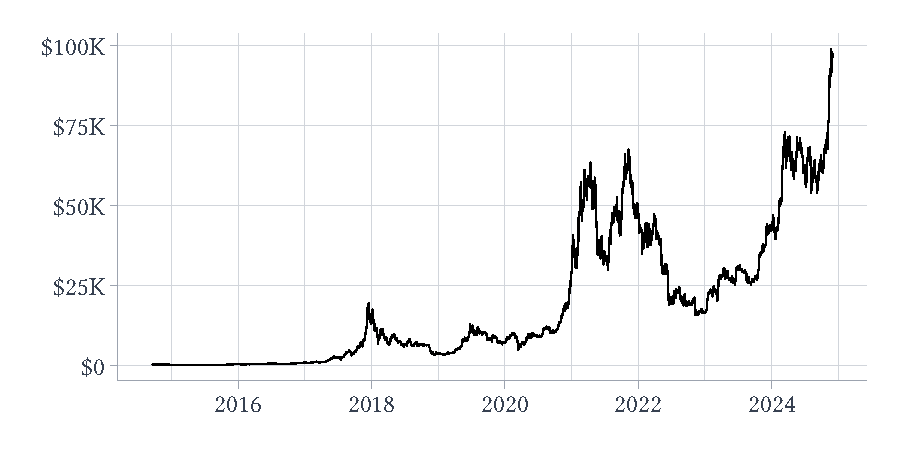
\includegraphics[width = 0.9\textwidth]{figures/bitcoin_raw.pdf}
  \end{center}
\end{figure}

\newpage
\begin{enumerate}
  \setcounter{enumi}{4}
  \item Say you take a sample of size 64 and estimate a sample mean of $\bar{X} = 40.6$. Additionally, you know the variance of $X$, $\sigma^2 = 24$. Construct a 95\% confidence interval for this sample mean. 

  \bigskip
  \item The following regression uses the ``College Scorecard'' which describes all U.S. colleges/universities. The outcome variable is the average earnings of students 10 years after they enroll. There are two covariates including \texttt{hbcu} which is an indicator if the college is a historically-Black college or univeristy and \texttt{share\_low\_income} which is the share of students considered `low income' and takes values between 0 and 1.
  \begin{codeblock}[{}]
OLS estimation, Dep. Var.: mean_earnings_10yr_after
Observations: 2,078
                  Estimate Std. Error   t value  Pr(>|t|)    
(Intercept)       65281.86    809.581  80.63656 < 2.2e-16 ***
hbcu::1           -6752.49    701.296  -9.62859 < 2.2e-16 ***
share_low_income -40604.40   1840.844 -22.05749 < 2.2e-16 ***
---
Signif. codes:  0 '***' 0.001 '**' 0.01 '*' 0.05 '.' 0.1 ' ' 1
  \end{codeblock}

  \begin{enumerate}[leftmargin = 2em]
    \item Interpret in words the estimated coefficient on the \texttt{hbcu} indicator. 
    
    \item Interpret in words the estimated coefficient on the \texttt{share\_low\_income} variable. Is a `one unit' increase a meaningful quantity in this case?
  \end{enumerate}
\end{enumerate}





\end{document}
